\documentclass[10pt]{academydoc}
\pagestyle{plain}

% Set Document Details
\doctype{tb} % spec, proc, tb (Specification, Procedure, Technical Bulletin)
\docname{Alternate ACES Viewing Pipeline User Experience}
\altdocname{Alternate ACES Viewing Pipeline User Experience}
% Sets the document name used in header - usually an abbreviated document title
\docnumber{TB-2014-013}
\committeename{Academy Color Encoding System (ACES) Project Committee}
\versionnumber{1.0.1}
\docdate{April 24, 2015}
\summary{
The majority of products that implemented pre-release ACES adopted an approach that combined the RRT and ODT into a single transform. It may useful to have one transform that has both ACES rendering components (from the RRT and ODT) that outputs the desired display colorimetry followed by a simple transform that converts that colorimetry into display code values. The ACES User Experience Working Group is developing an alternate UX proposal for products that wish to structure their viewing pipeline using this approach. This work is put forward for consideration as a possible recommended approach for a future ACES release.
}

% Document Starts Here
\begin{document}

\maketitle

% This file contains the content for the Notices
\prelimsectionformat	% Change formatting to that of "Notices" section
\chapter{\uppercase{Notices}}
%% Modify below this line %%

\copyright\the\year{} Academy of Motion Picture Arts and Sciences (A.M.P.A.S.). All rights reserved. This document is provided to individuals and organizations for their own internal use, and may be copied or reproduced in its entirety for such use. This document may not be published, distributed, publicly displayed, or transmitted, in whole or in part, without the express written permission of the Academy.

The accuracy, completeness, adequacy, availability or currency of this document is not warranted or guaranteed. Use of information in this document is at your own risk. The Academy expressly disclaims all warranties, including the warranties of merchantability, fitness for a particular purpose and non-infringement.

Copies of this document may be obtained by contacting the Academy at councilinfo@oscars.org.

``Oscars,'' ``Academy Awards,'' and the Oscar statuette are registered trademarks, and the Oscar statuette a copyrighted property, of the Academy of Motion Picture Arts and Sciences.

% This paragraph is optional.  Comment out if you wish to remove it.
This document is distributed to interested parties for review and comment. A.M.P.A.S. reserves the right to change this document without notice, and readers are advised to check with the Council for the latest version of this document.

% This paragraph is optional.  Comment out if you wish to remove it.
The technology described in this document may be the subject of intellectual property rights (including patent, copyright, trademark or similar such rights) of A.M.P.A.S. or others. A.M.P.A.S. declares that it will not enforce any applicable intellectual property rights owned or controlled by it (other than A.M.P.A.S. trademarks) against any person or entity using the intellectual property to comply with this document.

% This paragraph is optional.  Comment out if you wish to remove it.
Attention is drawn to the possibility that some elements of the technology described in this document, or certain applications of the technology may be the subject of intellectual property rights other than those identified above. A.M.P.A.S. shall not be held responsible for identifying any or all such rights. Recipients of this document are invited to submit notification to A.M.P.A.S. of any such intellectual property of which they are aware.

\vspace{10pt}
These notices must be retained in any copies of any part of this document. \newpage
% This file contains the content for the Revision History and 
\prelimsectionformat	% Change formatting to that of "Notices" section
\chapter{Revision History}
%% Modify below this line %%

\begin{tabularx}{\linewidth}{|l|l|X|}
    \hline
    Version & Date & Description \\ \hline
    1.0     & 05/10/2013 & Initial Version      \\ \hline
    1.1     & 08/02/2013 & Modify ACESproxy to handle negative ACES values \\ \hline
    2.0     & 12/19/2014 & Modify ACESproxy primaries, constrain to legal range \\ \hline
    2.0.1   & 04/24/2015 & Formatting and typo fixes \\ \hline
            &      &             \\ \hline
\end{tabularx}

\vspace{0.25in} % <-- DO NOT REMOVE
\chapter{Related Academy Documents} % <-- DO NOT REMOVE
\begin{tabularx}{\linewidth}{|l|X|}
    \hline
    Document Name & Description \\ \hline
    S-2008-001  & Academy Color Encoding Specification (ACES) \\ \hline
    S-2014-003  & ACEScc -- A Logarithmic Encoding of ACES Data for use within Color Grading Systems \\ \hline
    S-2014-004  & ACEScg -- A Working Space for CGI Render and Compositing \\ \hline
    & \\ \hline
    & \\ \hline
\end{tabularx} \newpage

\tableofcontents \newpage

% This file contains the content for the Introduction
\unnumberedformat	    % Change formatting to that of "Introduction" section
\chapter{Introduction} 	% Do not modify section title
%% Modify below this line %%

A goal of ACES 1.0 is to enable widespread adoption by encouraging consistent implementations in production and post-production tools throughout the complete film and television product ecosystem spanning capture to archiving. This is a very diverse set of tools, each used by professionals with different sets of skills. Furthermore, each manufacturer has established their own set of conventions for how to structure their user experience to best serve their market. Clearly, it is neither feasible nor appropriate for these guidelines to specify in minute detail every aspect of a user interface (e.g. ``all products must use a set of vertical drop-down menus labeled in 10-point Helvetica'').

That said, the feedback from users on the first wave of products implementing the pre-release versions of ACES has been clear in the need for guidelines. One common comment is that the implementations are so different, figuring out how to configure ACES in one product is of little help when configuring the next. For example, naming conventions are different for no apparent reason.

Another common concern is that the system is too reliant on acronyms and uses unfamiliar concepts (e.g., what is a ``reference rendering transform''?). Although some of these acronyms have become familiar within the inner circle of ACES product partners and early adopters, it must be acknowledged that the tolerance for these terms is much lower amongst the general population of industry professionals (e.g. how would one explain what an RRT is to an editor, CG animator, or anyone else without some color science background).

As the ACES project transitions from technical development to wider industry deployment and the release of Version 1.0, it is appropriate that we take a fresh look at how to portray the system to an audience that includes end-users in addition to engineers and color scientists. Although the technical terms and acronyms will continue to be used within the engineering community, these guidelines introduce a new set of terms intended to be simpler and more familiar to a wider set of users.

\note{This document provides naming conventions in English. However, it is recognized that for many products it will be necessary to translate these names into other languages to localize for various global markets.} \newpage

% This file contains the content for a main section
\numberedformat
%% Modify below this line %%
\chapter{Challenges}

In many implementations of pre-release ACES, products required users to select from a long list of transforms essentially consisting of the RRT combined with an ODT. The ODTs supplied with pre-release versions of ACES varied along the following characteristics:

\begin{itemize}
    \item released version of the CTL transforms
    \item display calibration aim
    \item cinema simulation mode vs. adapted mode
    \item target gamut limiting
    \item legal vs. full range
    \item forward and inverse transforms
\end{itemize}

Furthermore, we are introducing additional factors such as:

\begin{itemize}
    \item viewing environment
    \item target dynamic range (for HDR displays)
\end{itemize}

The factorial combinations of these transforms implies that it would be overwhelming to users to ask them to select from amongst dozens or even hundreds of possible transforms. Some principle must be found to organize them.

Further complicating matters is that the algorithms currently in use do not support all possible combinations of parameters (nor do all combinations even make sense as user options). For example, the target gamut limiting is very device specific. Likewise options for HDR video displays do not make sense for typical video displays or cinema projectors. So as with Input Transforms, it is not feasible to present the choices as a consistent and well-ordered set of parametric options.

Finally, the notion of an RRT + ODT and other aspects of the pre-releases are unique to ACES and become difficult in the context of products which simultaneously need to support other methods of color management.
% This file contains the content for a main section
\numberedformat
%% Modify below this line %%
\chapter{Structuring the choices}

Fundamentally, there are two main decisions to be made by the user: first, what device is being used to display the images; and second, how are the images to be viewed. As is the goal in UX design, the first decision, the display, is something that is intuitively obvious and expected.

The second decision is less obvious but there is precedent for it. For example, many users are already familiar with the notion that logarithmically encoded images (e.g. negative-film scans) require some type of transformation (e.g. a print-film emulation) in order to be viewed correctly.

By splitting the decision-making process into two steps, rather than requiring the user to select from a long list with M x N choices, they are able to make two separate choices, each from a much shorter set of options (of length M and N). (This is an over-simplification of the system, but hopefully the concept is clear.)

This particular decomposition into Viewing and Display Transforms allows ACES to fit into some color management UX models that are already in common use. For example, OpenColorIO already structures its viewing pipeline into View and Display choices. 

Another example are the products that use ICC-based color management. These products make use of the ICC monitor profile that is ubiquitous within the Mac and Windows operating systems and which convert desired colorimetry to display code values. Structuring the choices as View and Display allows ACES to be more easily integrated into ICC-based products.
% This file contains the content for a main section
\numberedformat
%% Modify below this line %%
\chapter{Filtering the available View Transforms}

Metadata is now added to the ACES transforms which include a unique transform identifier. Additionally, metadata could be added to Display Transforms to include the IDs of the View Transforms for which they are authored. For example, a digital cinema projector and an HDR monitor will be authored using different View Transforms. For a typical Display Transform, this will be a list of 1-2 View Transforms. For example, in the case of a broadcast monitor there are two: one for video mastering mode and another for simulating the D60 white point of the cinema mode (e.g. for on-set use). So once the Display Transform has been selected, the application should filter the list of ACES View Transforms to only the appropriate ones (usually just 1-2).
% This file contains the content for a main section
\numberedformat
%% Modify below this line %%
\chapter{The role of the RRT}

Please note that although the RRT acronym is not used in the suggested terminology, it still remains an essential piece of the engineering and conceptual model of ACES. The role of the RRT is to define the baseline ACES rendering. Even though there are multiple Viewing Transforms for the viewing environments and classes of display (e.g. standard and extended dynamic range), these are all designed to match the RRT to the extent possible. This is what gives the ACES renderings a consistent appearance across a wide range of viewing environments and display technologies.
% This file contains the content for a main section
\numberedformat
%% Modify below this line %%
\chapter{Terminology}

These terms should be introduced:

Viewing Transform (or View Transform) -- Generally, a color transformation that converts values from a working space into colorimetry for a display device. Specifically in this context, the Viewing Transform is what contains the Academy-supplied algorithms for converting scene-referred ACES values into colorimetry for a given viewing environment and class of display.

Display Transform -- A color transformation that converts colorimetry intended to be reproduced on a display into the code values that must be sent to the device.
% This file contains the content for a main section
\numberedformat
%% Modify below this line %%
\chapter{Mapping from the engineering-centric to user-centric terms}

There is not a one-to-one mapping of the RRT to a View Transform or from an ODT to a Display Transform. 

\autoref{fig:conceptualModel} shows the ACES viewing pipeline using the engineering-centric LMT, RRT, and ODT terms. \autoref{fig:userCentricModel} shows how the recommended terms apply to the same underlying blocks being used in \autoref{fig:conceptualModel}. Note that both pipelines produce exactly the same numerical results.

Two new engineering-centric acronyms are used here since there is a need to be able to refer to the part of the ODT which contains the Academy-developed part of the algorithm (which is key to the look of the system), from the more typical conversion from colorimetry into code values for a given display.

Target Conversion Transform (TCT) -- The TCT may be thought of as the part that ``fits'' the idealized colorimetry from the RRT into what is appropriate for a viewing target. A viewing target consists of a family of display devices (i.e. devices which have similar dynamic range and gamut characteristics) and associated viewing environment.

Display Encoding Transform (DET) -- The DET is simply a conversion from colorimetry into the code values necessary to produce that colorimetry on a given device. It is similar to an ICC monitor profile.

\begin{figure}[htbp]
\begin{center}
    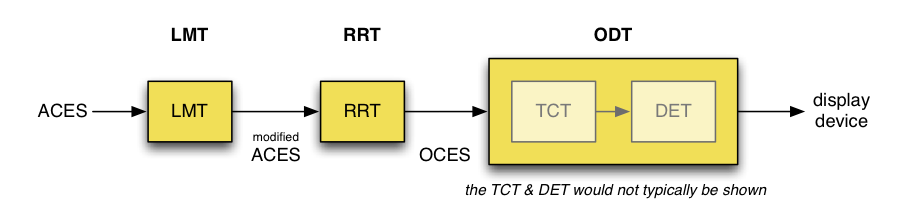
\includegraphics[width=\textwidth]{conceptualModel.png}
\caption{The conceptual model of viewing ACES}
\label{fig:conceptualModel}
\end{center}
\end{figure}

\begin{figure}[htbp]
\begin{center}
    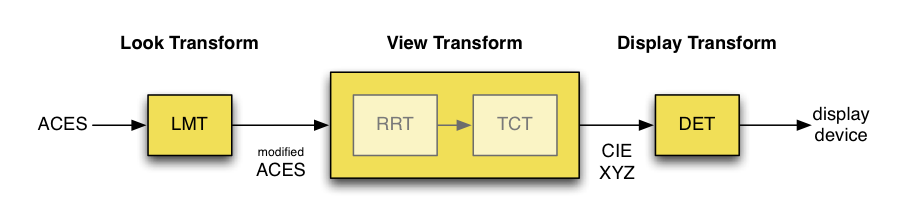
\includegraphics[width=\textwidth]{userCentricModel.png}
\caption{Engineering-centric ACES viewing pipeline along with the user-centric model}
\label{fig:userCentricModel}
\end{center}
\end{figure}


\end{document}